\documentclass{article}
\PassOptionsToPackage{numbers,sort&compress}{natbib}
\usepackage[preprint]{neurips_2026}
\usepackage{graphicx}
\usepackage{booktabs}
\usepackage{amsmath}
\usepackage{url}
\usepackage[hidelinks]{hyperref}
\usepackage{microtype}

\title{An Unconditional VAE for Chest X-Ray Generation}
\author{
  Cai Xinyan\\
  ECE 285: Deep Generative Models, University of California, San Diego
}

\begin{document}
\maketitle

\begin{abstract}
We implement a convolutional variational autoencoder (VAE) in PyTorch and train one unconditional model on pooled NORMAL and PNEUMONIA chest X-rays, following the instructor's clarification. We use a fixed training/validation split and hold out the original test set. The model reaches a stable validation loss and generates recognizable but smooth radiographs. We report training settings, the loss curve, Inception Score (IS), Fr\'echet Inception Distance (FID), and sample images.
\end{abstract}

\section{Data and method}
The dataset contains 5,856 images from Kaggle and the Mendeley collection by Kermany et al. [1]. We used a public mirror that reports unchanged files and splits. After pooling labels, we split the original 5,216-image training folder into 4,694 training and 522 validation images (seed 42). The original 624-image test folder was held out. We did not use the separate 16-image validation folder.

Images were converted to grayscale, resized to $128\times128$, and scaled to $[0,1]$. The encoder has five stride-2 convolution blocks (32, 64, 128, 256, and 512 channels). Linear layers predict a 128-dimensional Gaussian latent distribution. A mirrored transposed-convolution decoder produces pixel logits. We minimize summed Bernoulli reconstruction loss plus KL divergence to a standard normal prior.

\begin{table}[h]
\centering
\small
\caption{Hyperparameters and selected run settings.}
\label{tab:settings}
\begin{tabular}{ll}
\toprule
Setting & Value\\
\midrule
Input size / channels & $128\times128$ / 1\\
Latent dimension & 128\\
Optimizer & Adam, learning rate $3\times10^{-4}$\\
Batch size & 64\\
Maximum epochs / patience & 150 / 18\\
LR scheduler & Reduce on plateau (patience 6, factor 0.5, min $10^{-5}$)\\
Train / split / sample seed & 43 / 42 / 2026\\
Compute & NVIDIA A100-SXM4-80GB, 22.3 min\\
\bottomrule
\end{tabular}
\end{table}

The best checkpoint was chosen by validation negative ELBO: epoch 120, with loss 9,426.60 per image. Training stopped at epoch 138 after 18 epochs without improvement. A second seed and a 256-dimensional latent variant were also tried; seed 43 had the lowest validation loss (9,426.60 vs. 9,426.81 and 9,427.19). Test scores were not used for selection.

\begin{figure}[t]
\centering
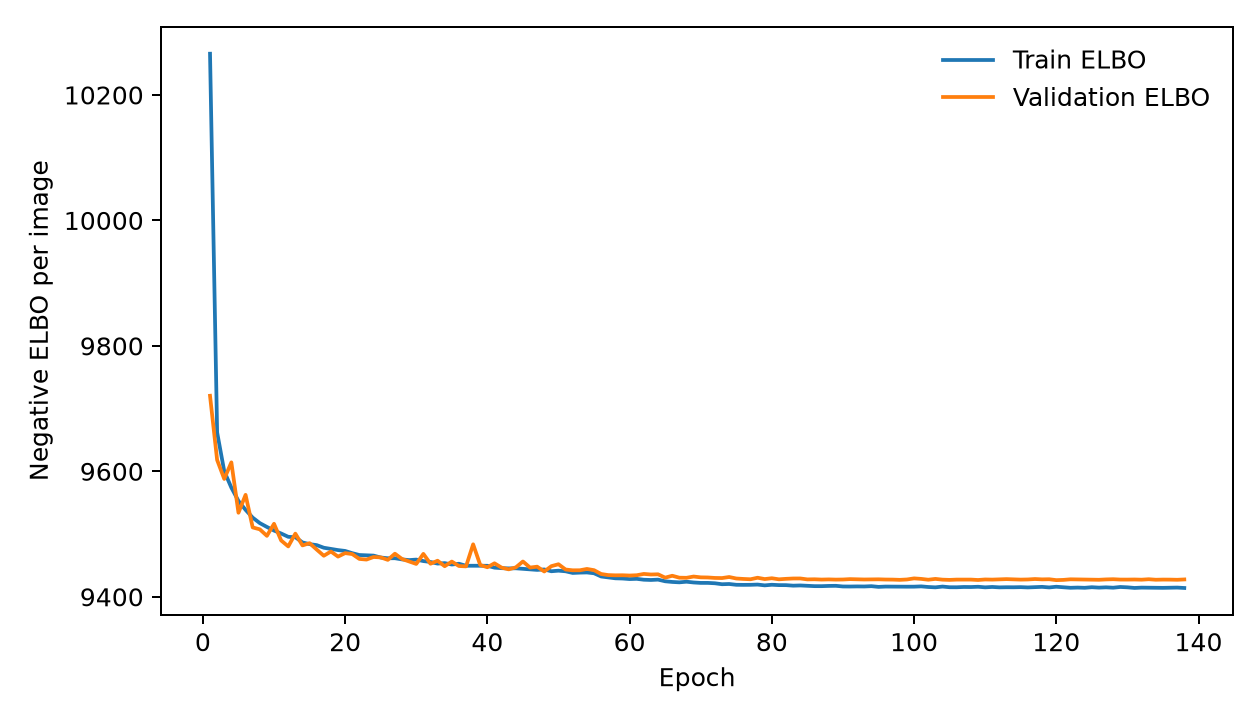
\includegraphics[width=0.55\linewidth]{figures/loss_curve.png}
\caption{Training and validation negative ELBO per image. The objective falls rapidly at first and then flattens; small later changes are consistent with convergence to a plateau. The epoch-120 checkpoint had the best validation value.}
\label{fig:loss}
\end{figure}

\section{Evaluation and results}
We use PyTorch-Ignite Inception-v3 metrics [2] with 624 generated samples (seed 2026) and 624 held-out test images.

\begin{figure}[t]
\centering
\begin{minipage}[t]{0.43\linewidth}
\vspace{0pt}
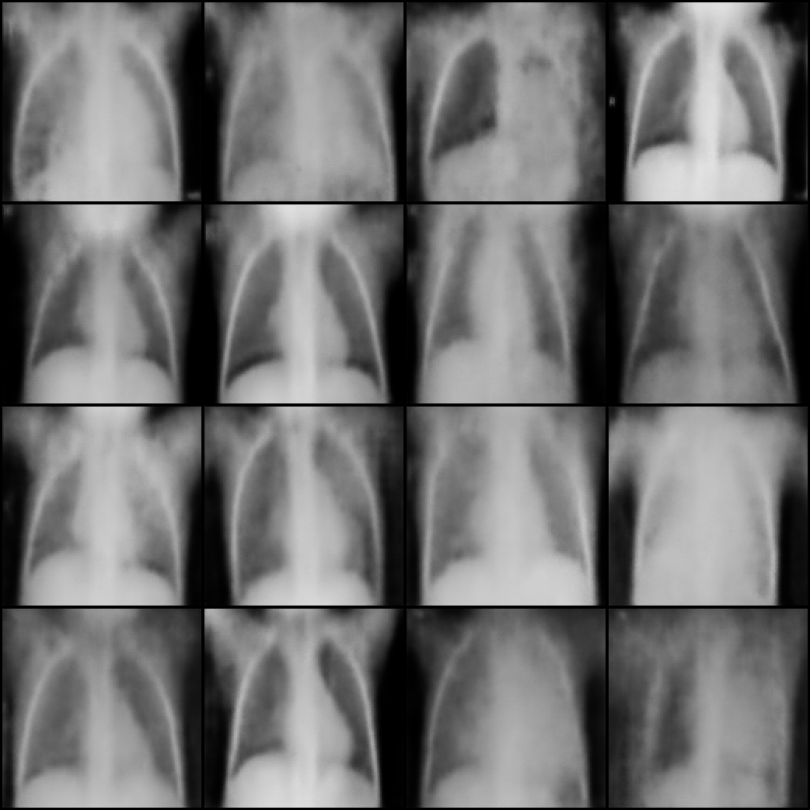
\includegraphics[width=\linewidth]{figures/samples_4x4.png}
\end{minipage}\hfill
\begin{minipage}[t]{0.51\linewidth}
\vspace{0pt}
\centering
\small
\begin{tabular}{lc}
\toprule
Metric & Result\\
\midrule
Inception Score (IS) & 1.926\\
FID & 0.162\\
Images per distribution & 624\\
\bottomrule
\end{tabular}

\vspace{0.6em}
\raggedright
\footnotesize
IS uses generated samples; FID compares test features. Grayscale inputs are repeated as RGB and resized to $299\times299$. The scores are approximate, not clinical measures.
\end{minipage}
\caption{Sixteen prior samples (left) and held-out test metrics (right). Chest outlines are recognizable, but fine details remain smooth.}
\label{fig:results}
\end{figure}

\section{Analysis}
The curve plateaus after rapid early improvement. Samples vary and capture broad chest anatomy, but ribs and lung details are blurred. Square resizing and the $128\times128$ pixelwise Bernoulli model limit fine detail. Since labels are pooled, the model cannot control whether a sample resembles a NORMAL or PNEUMONIA image.

IS and FID are approximate: Inception is trained on natural images, and FID depends on features and sample count. These 624-sample scores are not clinical measures. The synthetic images must not be used for medical decisions. Code, history, metrics, and all 64 samples accompany this report.

\begin{thebibliography}{9}
\small
\bibitem{data}
D. Kermany, K. Zhang, and M. Goldbaum. \emph{Labeled OCT and Chest X-Ray Images for Classification}. Mendeley Data, 2018. Dataset: \href{https://www.kaggle.com/datasets/paultimothymooney/chest-xray-pneumonia}{Kaggle}; mirror: \href{https://huggingface.co/datasets/ahulikal/chest-xray-pneumonia-mirror}{Hugging Face}. CC BY 4.0.

\bibitem{ignite}
PyTorch-Ignite. \emph{GAN evaluation using FID and IS}. \href{https://pytorch-ignite.ai/blog/gan-evaluation-with-fid-and-is/}{Tutorial}.
\end{thebibliography}

\end{document}
